%%% LEXICON %%%
% Block: A literal block on the workspace (like a move block)
% Chain: A series of connected blocks.
% Program: All chains on the workspace.
% Workspace: The canvas where blocks are.
% Cognitive Load: The amount of thinking needed to complete a task.
% Redundancy Effect: When redundant information causes a user to understand content less, than if the redundant content was removed
% Grammar: The structure of language that is recognized by our speech recognition
% Utterance: What is said by the user
% Recognition: What the speech recognition "hears" from the user
% Correction: The outcome of our correction algorithm on the recognition
% Toolbox: Where the available blocks can be found 
% Action: A manipulation performed by mouse or keyboard
% Command: A manipulation performed by speech

\documentclass[]{article}

\usepackage{wrapfig, algorithm, algpseudocode, amsmath, amssymb, xspace, mathalfa, graphicx}
\graphicspath{ {images/} }

% Example of this command
% \fig{MYFIGNAME001}{my caption}{size}
% See figure \ref{fig:MYFIGNAME001}

\newcommand\fig[3]{
\begin{figure}
  \begin{center}
  \includegraphics[#3]{images/#1}
  \caption{#2} 
  \label{fig:#1}
  \end{center}
\end{figure}
}

% Blank
\newcommand{\uline}[1]{\rule[0pt]{#1}{0.4pt}}

\def\sg{\textsc{SpeechGames}}

\title{\sg: Voice Programming in Computer Science Education}

\begin{document}
\maketitle

\begin{abstract}
  We introduce the $\sg$ platform for exploring topics in computer science
  education.
  % TODO
\end{abstract}

\section{Introduction}

% \subsection{What is the goal of the project? What problem does it solve?}
% \subsection{Who is meant to benefit?}

There is tremendous interest in computer science education.
% cite hour of code
\sg~is a platform
that may be used to explore topics in computer science education for children
who may be suffering from disabilities by means of a voice interface to the
Blockly coding environment. The may help children who are unable to use a mouse
and keyboard interface.

% Our goal is to create a voice enabled platform that uses machine learning to allow 
% anyone to learn the fundamentals of computer science. Currently, we seek to reduce the amount
% of cognitive load required to be learn programming concepts, which would give more 
% students opportunities in computer science. 
% \\ 
% Voice programming looks to benefit both new and experienced programmers.  
% Google Blockly is a simple language that allows us to create a robust programming grammar 
% that can be used of people of all ages. In addition to discovering solutions to voice 
% recognized programming, our project will help teach people who are unable to use a traditional mouse and keyboard.

% \subsection{What are the results or outcome of the project?}

% TODO We need something more experiential

In this technical report, we shall first describe our design principles for
$\sg$, following guidelines proposed by cognitive load theory worked out in
educational psychology and computer science education. Then we will go on to
describe components of our architecture, from the programming environment to the
speech recognition interface. After we've described the building blocks, we will
detail algorithmic work to improve usability. And then we will proceed to
discuss related and future work.

\section{HCI Principles}
% \subsection{What HCI principles were kept in mind in the design of our system?}
% \subsection{How did those HCI principles influence our design decisions?}
Cognitive load is the total amount of mental effort being used in the working
memory~\cite{sweller1988cognitive}. Reducing cognitive load has been linked to
improved educational outcomes~\cite{kalyuga2010facilitating}, and hence was a
guiding principle in designing our educational platform.

Cognitive load theory distinguishes between three different types of load:

\begin{itemize}
  \item \textbf{Intrinsic load.}
  \item \textbf{Extraneous load.}
  \item \textbf{Germane load.}
\end{itemize}
% TODO Define these and point out relevance for what we're doing (germane load:
% motivation and interest)

\cite{rebetez2006control} further identifies a series of effects to serve as
guidelines for creating learning materials:

\begin{itemize}
  \item \textbf{Redundancy effect}
  % TODO
\end{itemize}
   
Speech recognition presents particular challenges for designing effective
educational materials. \cite{Shneiderman:2000:LSR:348941.348990} argues that
speech input/output consumes cognitive resources in short-term and working
memory, these effects being mitigated in applications with a limited vocabulary
and constrained semantics.

\section{Blockly}
% \subsection{What is the Blockly environment?}
% \subsection{What is the goal of the Blockly project?}
Google Blockly is a JavaScript library that creates a visual block programming 
environment where core computer science logic can be taught, such as conditionals and 
looping. Blockly is run in the web browser, which gives the opportunity for mobile use. 
We chose Google Blockly over other block based languages due to its easy to work with and 
has a customizable API.

% \subsection{How are blocks arranged horizontally? What language do we use to describe this?}
% \subsection{How are blocks arranged vertically? What language do we use to describe this?}
% \subsection{Is just one chain of blocks allowed or several?}
% \subsection{If several, how are they executed?}
% \subsection{How does the user typically interact with Blockly?}
% \subsubsection{What's the medium (hint: mouse)?}
% \subsubsection{What actions are available?}
% \subsubsection{How can we group them into categories?}
% \subsubsection{How does moving blocks work?}
% \subsubsection{How does deleting blocks work?}
% \subsubsection{How does connecting blocks work?}
% \subsubsection{How does separating blocks work?}
% TODO: Define 'actions' in this section

\fig{workspaceDiagram.jpg}{Google Blockly workspace diagram}{width=7cm}

Let us introduce some terminology here that would be used extensively in the
paper moving forward. Blockly has the concept of a \textbf{workspace}, as shown
in \textbf{Figure~\ref{fig:workspaceDiagram.jpg}}. This is the space where all
the blocks that need to be executed in the program are located. A \textbf{chain
  of blocks} refers to a series of vertically connected blocks in the workspace.
Vertically connected blocks are executed sequentially. In Google Blockly, it is
also possible to several unconnected chains of blocks in the workspace. These
chains are executed in order of the coordinates of their topmost block. A menu
to the left of the workspace holds the available block types for a program. We
will refer to this menu of available block types as the \textbf{toolbox}. In
order to move blocks from the toolbox to the workspace, users must click and
drag using a mouse in a traditional Blockly setting.

The toolbox is where all the allowed blocks for a particular program can be found. Google Blockly has a large library of blocks, which can be grouped as:
\begin{itemize}
  \item$\textbf{Logic}$: if statements and equality testing
  \item$\textbf{Loops}$: while loops, for loops, for-each loops and break statements
  \item$\textbf{Math}$: incrementing variables, summing numbers, randomizing numbers and other basic math and geometry operations.
  \item$\textbf{Text}$: displaying text, appending text, searching through text, substring, printing and prompting
  \item$\textbf{Lists}$: creating a list with variables, length, testing if empty and searching through a list
  \item$\textbf{Color}$: changing the color and random coloring
  \item$\textbf{Variables}$: creating a variable, initializing it and modifying its value
  \item$\textbf{Functions}$: a chain of blocks with a name and a possible return value
\end{itemize}

\section{Speech}

% TODO: Define 'commands' in this section -- done

%\subsection{Why did we decide to model speech using a fixed grammar?}
To reduce cognitive load, we focused on creating a concise and fixed grammar, 
meaning there is only one way to say a command, which is a term we use to 
describe a manipulation performed by speech. While speech recognition can be 
used for a conversation style of programming, we wanted to mimic the standard 
idea that computer languages have rigid grammars. 

%\subsection{What choices did we make as we designed that grammar?}

To create a rigid grammar, we focused on making the grammar as simple as
possible. We employed a guiding principle of \textbf{syntactic parsimony}. That,
there ought only be one command in the grammar per action in the workspace. For
this reason, the grammar includes no optional or choice elements. No synonyms
are allowed for the main verbs (get, delete, change, connect, separate) of the
sentences of the grammar. We also disallowed variability on prepositional phrase
location. For example, we only allow ``Change left in block 1 to right'' and not
``Change left to right in block 1.'' We were also guided by a principle of
\textbf{semantic parsimony}. The commands ``Move block 2 under block 1'' and
``Move block 1 under block 2'' for example might be equivalent operations, but
due to semantic parsimony, we only allow moving blocks \emph{under} one another.

%\subsection{What commands are available in that grammar?}
%Users must refer to blocks as the block number that is shown on the block\\
%\textbf{Users can move blocks in 2 ways}:
%\begin{itemize}
%\item \textbf{Connect block $<$ID$>$ under block $<$ID$>$}: allows user to move blocks and chains of block under any block or chain of blocks
%\item \textbf{Connect block $<$ID$>$ inside block $<$ID$>$}: allows user to move block and chains of blocks inside of a repeat block
%\end{itemize}
%\textbf{delete block $<$ID$>$}: deletes a block,  unless the block is the head of a chain of blocks, then this command deletes the entire chain of blocks.

% TODO: I'm not sure what this means exactly
The user has the following commands: 
\begin{itemize}
  \item Add  - ``get a \uline{1cm} block''
  \item Connect - ``connect block \uline{.5cm} under block \uline{.5cm}''
  \item Connect inside - ``connect block \uline{.5cm} inside block \uline{.5cm}''
  \item Separate - ``seperate block \uline{.5cm}''
  \item Change field - ``change \uline{.5cm} in block \uline{.5cm} to \uline{.5cm}''
  \item Delete - ``delete block \uline{.5cm}''
  \item Run program - ``run the program''
  \item Next level - ``go to the next level''
  \item Stay on level - ``stay on this level''
\end{itemize}
\subsection{How do the user interface commands described earlier map to the
commands in the grammar?}


\section{Turtle}

% \subsection{What is the turtle game?}
% \subsection{What set of blocks are available to complete the game?}
% \subsection{What do these blocks do?}
% \subsection{Why is the game divided into levels?}
% \subsection{How do the levels serve to teach different programming concepts?}

\fig{turtle_workspace.jpg}{Turtle workspace diagram}{width=4cm}

In order to implement the voice-programming interface using Blockly, we decided to use Turtle.
Turtle is a Blockly game, that contains a turtle that can be moved around using a small subset of commands (blocks). 
The objective of the game is to make the turtle trace a particular path shown to the user, using only the provided blocks in the toolbox.
Turtle is one of many Blockly games that we could have chosen in combination with Google Blockly and our speech recognition, but chose it for its simplistic design.

\begin{itemize}
  \item $\textbf{move}$: moves the turtle forward
  \item $\textbf{turn}$: turns the turtle, can decide between left or right turning and angle of turning  1, 45, 72, 90, 120, 140 degrees
  \item $\textbf{repeat}$: repeatedly executes the blocks inside it, can decide to repeat either 2, 3, 4, 5 or 360 times
  \item $\textbf{pen}$: can decide between up/down, up stops the turtle from drawing a line, down makes the turtle's movements draw lines again
\end{itemize}

Turtle evenly divides computer science concepts into levels in order to reduce the cognitive load of the learner.
Each individual level reinforces previously learned topics, while introducing new ones simultaneously. 
An example of a couple of consecutive levels would be as follows:
\begin{enumerate}
  \item User is exposed to how to move the turtle forward and also turn the turtle to make a square. In order to make the square, the user is only give move and turn blocks, meaning they need four move blocks and three turn blocks to complete the task.
  \item User is given a repeat block in the toolbox. Now the user is tasked at completing the same task as before, but with only using one repeat block, one move block and one turn block.
\end{enumerate}

A user has now, in two levels, been first introduced to the mechanics of moving and turning the turtle in the Google Blockly environment and then naturally transitioned into loops. Since the task is simply ``create a square'', it is not too difficult to utilize the new blocks provided, given the knowledge of previous levels.

\section{Speech recognition}
%\subsection{How do we perform the speech recognition? What do we use?}
%\subsection{What tradeoffs are there in our decision by comparison to alternatives? What was gained and what lost?}

We perform speech recognition using the Webkit Speech API in Google Chrome. The API provides us with the user's speech, as understood by the speech recognition engine, in text form. We chose this option over CMU's Sphinx because we wanted to get better recognition and the Google Speech API has been trained on a lot more data compared to CMU's Sphinx engine which we could train on a limited and non-representative set of data that we would generate. Google's Speech API is also easier to use and available in other web browsers (since this is primarily a web application).

\section{Suggestions}

%\subsection{Why do we give suggestions to the user? What HCI principle is behind this?}
%\subsection{What is basis on which a speech suggestion is made? What circumstances trigger it?}
%\subsection{What are the limitations of the current method and what future work might improve upon it?}
%\subsection{Show an example of the suggestions box and workspace before and after an operation}

% TODO Why do we have a suggestions list? (Well, because of the fixed grammar.
% The user is not given any training in the grammar per se.) -- done

% TODO Point out that the user might get the impression that we are giving
% suggestsions to solve the problem while we are only giving hints on how to use
% the grammar. -- done

% TODO Fix "novel algorithm", reference alg -- done
% TODO May want to shorten Alg 1 vars and describe it in text -- done
% TODO Fix quotes -- done
% TODO Why? What's the problem with always correcting? If the user says
% something utterly unrelated, we still correct it! -- done

We provide the user a list of suggestions to teach them the grammar. We do this because the grammar is a rigid, fixed grammar. Furthermore, we provide these suggestions because we don't give any training in the grammar to the user. Instead, we hope that they can pick it up by following the suggestions. The suggestions mechanism provides generic suggestions, not specific to the block IDs or the workspace. We do not suggest how the user should solve the program, as the user might mistakenly believe. Instead, we simply teach them how to use the grammar. However, the appearance of particular suggestions is triggered by certain states of the workspace. For example, when an empty repeat block is on the canvas, we suggest that the user ``Connect block 2 inside block 1'' with these exact block IDs, regardless of what the block ID of the repeat block is. Finally, we provide an example in Table \ref{SuggestionsBeforeAndAfter} of the suggestions box with the corresponding workspace before and after adding the first block. We modify the suggestions list when we believe it could be useful for the user. For example, when there is a repeat block on the canvas, we suggest that the user connects a block inside of the repeat block, to make use of the repeat block. However, our current suggestions system is quite limited.\\
\begin{table}
	\caption{Example of suggestions before and after adding the first block to the workspace.}
	\label{SuggestionsBeforeAndAfter}
	\begin{tabular}{cccc}
		\hline
		when & workspace & suggestions \\\hline
		\\
		before & 
\includegraphics{suggestions_before_workspace.jpg} & 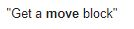
\includegraphics{suggestions_before.jpg} \\\hline
		\\
		after & 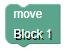
\includegraphics{suggestions_after_workspace.jpg} & 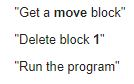
\includegraphics{suggestions_after.jpg} \\\hline
	\end{tabular}
\end{table}

\section{Corrections}
%\textit{Utterance:} A single command given by the programmer\\
%\textit{Recognition:} What the speech reognition software recogizes an utterance as\\
%\textit{Correction:} The proposed utterance given a recognition, calculated using correction algorithm\\

%\subsection{Give an example of a common recognition error that falls out of the grammar}
%\subsection{What algorithm was used to correct recognition?}
As previously described, we use the Google speech API built into Google Chrome 
to capture user commands. However, the API has a hard time understanding 
commands from our grammar. We hypothesize that the API expects ordinary 
English, and as a result, phrases like ``get a turn block'' or ``change 4 in 
block 3 to 5'' are often recognized incorrectly by webkitspeechcrecognition. We 
developed Algorithm \ref{CorrectionAlgorithm} to correct incorrectly recognized 
phrases (``recognitions'') to what we hope are the intended commands 
(``utterances''). 

The correction algorithm first takes in a recognition $r$, a workspace $W$, and 
a max modification factor (described later) $\lambda$. First, the recognition 
$r$ is converted into a phoneme sequence $\rho$ using a modified version of 
CMU's pronouncing dictionary~\cite{rudnicky2015cmudict}. Then we generate a set 
$C$ of all possible commands that a user can specify given the workspace. For 
each command $c$, we convert it into a phoneme sequence $\gamma$ and compute 
its edit distance $e$ to $\rho$. We iterate over $C$ to find the minimum edit 
distance $e^*$ (breaking ties arbitrarily) and corresponding minimum edit 
distance command $c^*$.  
% TODO Cite CMU pronouncing dictionary -- done
% TODO Introduce some simple notation (and use same notation in algorithm 1) -- 
%done

Furthermore, if $\mu$ is too far from the original recognition sequence $\rho$, 
we reject the correction  $\mu$ and notify the user that we didn't understand 
their command. We added this feature to avoid using a ``correction'' from a 
completely unrelated sentence picked-up or recognized by the speech API. Our 
notion of ``too far'' is satisfied when$$ e^* > \lambda * length(\rho)$$ As 
such, 
there is no fixed maximum number of edits, as this could give 
different performance for different string lengths. 
% TODO make this math -- done?
\begin{algorithm}
	\caption{Correction Algorithm}\label{CorrectionAlgorithm}
	\begin{algorithmic}[1]
		\Procedure{Correct}{r, W, $\lambda$}
		\State $\rho \leftarrow stringToPhoneme(r)$
		\State $C\leftarrow generatePossibleCommands(W) $
		\State $e^* \leftarrow \infty$
		\State $c^* \leftarrow r$
		\State $\gamma^* \leftarrow \rho$
		\For{$c$ in $C$}
			\State $\gamma \leftarrow stringToPhoneme(c)$
			\State $e \leftarrow findMinEditDist(\rho, \gamma)$
			\If{$e < e^*$}
				\State $e^* \leftarrow e$
				\State $c^* \leftarrow c$
				\State $\gamma^* \leftarrow \gamma$
			\EndIf
		\EndFor
		\If{$e^* \leq \lambda * length(\rho)$}
			\State \Return{$c^*$}
		\Else
			\State \Return{$r$}
		\EndIf
		\EndProcedure
	\end{algorithmic}
\end{algorithm}

\subsection{Correction Algorithm Parameters}
The correction algorithm requires the following parameters to run:-
\begin{itemize}
\item \textbf{Recognition}: The recognition of the utterance by the speech API.
\item \textbf{Workspace}: The state of the workspace that contains information about the numbers and types of blocks currently present on the workspace.
\item \textbf{Maximum Modification Factor}: The maximum percentage of modification (i.e. correction) allowed to the original recognition. The methodology to get calculate this number, is described in section 8.2.
\end{itemize}

\subsection{Calculation of Maximum Modification Factor}

\subsubsection{Data Collection}
The data was gathered manually by speaking into the speech engine and recording the utterance, recognition and correction (if it exists) in text form.
The correct and incorrect utterances, along with their recognitions and corrections were stored as CSV files. 
\subsubsection{Statistical Procedure}
The data containing the accuracy corresponding to each threshold value from 0.00 to 1.00 (with a step size of 0.01) was collected by running the analysis on both positive and negative data examples.

For the correct examples, the accuracy was obtained by counting the total number of correct corrections. In other words, we need to count the total number of times the recognition was corrected to the original utterance. For the incorrect examples, the accuracy was obtained by counting the total number of times corrections were not made - since corrections are always valid, mapping an incorrect utterance to a valid command is not correct.

Lastly, the maximum modification factor was calculated by using the threshold value that corresponded to the maximum average accuracy of the positive and negative examples. It is important to note that the average was calculated by weighing the categories equally, and not the examples.

\subsubsection{Limitations}
\begin{enumerate}
\item We had approximately 100 positive examples and 200 negative examples, and this is not the expected distribution of real-world data. In practice, we would expect a lot more positive examples than negative.
\item The negative examples were mostly random utterances that might be picked up by the microphone in a loud environment. In other words, these utterances didn't even come close to being recognized as a valid speech command. While this data might be useful when a lot of vocal activity is going on around the user, this does not serve any purpose in adapting the speech recognition to a user that is using the speech interface in a quiet environment (which is the expected behavior).
\item Sample size of approximately 300 examples is low.
\end{enumerate}
\subsection{Give an example of a common case that the corrections algorithm, as currently implemented, fails on}

\section{Layout}

%\subsection{How are commands interpreted visually?}
%\subsection{Where do new blocks go?}
%\subsection{How are blocks reordered when one is moved?}
%\subsection{What happens if the user runs out of space on the workspace?}
%\subsection{Describe the layout algorithm in pseudocode}
%\subsection{Show an example of the a before and after with the layout algorithm}
%\subsection{Are there any cases that currently give problems for the layout algorithm?}

As the user writes a program, certain locations on the workspace fill with blocks.
This presents a challenge: what should happen when blocks overlap with one another?
For our system to be practically useful, it must avoid introducing such visual impairments,
which may prevent the user from issuing commands (e.g. if they cannot see a block ID)
or which may introduce unnecessary cognitive load.

Blockly by default places new blocks at the top left of the workspace, even if the new block
will overlap an old block. Similarly, when Blockly connects one block to another, the resulting chain
might overlap another chain.

We devise simple layout algorithms for each case. To make this formal, we view
the workspace as a 2D plane $W$ where the origin is the top left corner, the $x$ axis ranges from 0
to $\textsc{Width}(W)$, and the $y$ axis ranges from 0 to $\textsc{Height}(W)$.
Let $B$ denote the set of blocks on the workspace and let $m$ denote a small, constant margin.
In our implementation, we choose $m = 20$ (pixels) because it is small enough to preserve space
on the workspace, and large enough to prevent Blockly from automatically connecting nearby blocks.

\textbf{Adding Blocks} We place new blocks by finding the vertically lowest free
position on the workspace and placing the new block there, exactky $m$ pixels right of
the toolbox. This is summarized by Algorithm~\ref{alg:place}.

\textbf{Moving Blocks} Suppose the user has just connected one block to another, and the
resulting chain now overlaps $n$ chains. We repair the layout by moving the $n$ conflicting
blocks individually via Algorithm~\ref{alg:relayout}. 

\begin{algorithm}[H]
\caption{Place New Block}\label{alg:place}
\begin{algorithmic}
\Procedure{PlaceNewBlock}{$B, m$}
\State $\ell \gets m$ \Comment{stores lowest $y$ on the workspace}
\For{$b \in B$} 
	\If{$y_b + \textsc{height}(b) \ge \ell$}
		\State $\ell \gets y_b + \textsc{height}(b) + m$
	\EndIf
\EndFor
\State \Return $(m, \ell)$
\EndProcedure
\end{algorithmic}
\end{algorithm}

\begin{algorithm}[H]
\caption{Relayout Existing Block}\label{alg:relayout}
\begin{algorithmic}
\Procedure{Relayout}{$b, B, W, m$}
\State $x \gets m$
\While{$x < \textsc{width}(W)$}
	\State $y \gets m$
	\While{$y < \textsc{height}(W)$}
		\If{$\textsc{CanMoveWithoutConflict}(b, (x,y))$} 
				\State $\textsc{Move}(b, (x,y))$
		\EndIf
		\State $y \gets y + m$
	\EndWhile
	\State $x \gets x + m$
\EndWhile
\State $\textsc{Move}(b, (m,m))$
\EndProcedure
\end{algorithmic}
\end{algorithm}

\section{Related Work}

Speech interfaces for programming tasks have a long history, dating back to the
beginning of speech recognition research \cite{bolt1980put}.

The bulk of work aims to improve the productivity of professional developers
using IDEs through speech. The first body of work here tends to specify its
method to a particular programming language. For example,
\cite{Begel05programmingby} creates a grammar for a language, Spoken Java, which
is syntactically similar to Java, with a goal of disambiguating natural language
utterances. \cite{desilets2006voicecode} uses a set of rules to trasncribe
dictation results into fragments of code. \cite{shaik2003speechclipse}
constructs a speech plug-in focused more on the IDE's control than its language.
And \cite{gordon2011developing} designs a programming language from the ground
up for the purpose of being developed through a speech interface.
\cite{hubbell2006voice} proposes a voice-activated syntax-directed editor.

A second group uses voice and other modalities, such as gesture and
eye-tracking, to control aspects of the IDE which need not be language-specific.
\cite{delimarschi2014enabling} maps human voice and gestures are mapped to IDE
commends using hardware sensors for Microsoft Kinect. \cite{glucker2014eyede}
adds eye-tracking control to IDEs.

The question of education for motorically challenged children has been
investigated in \cite{wagner2012programming} where a speech-based IDE was built
atop Scratch. Their grammar focuses around manipulation of the GUI elements of
the Scratch editor rather than the semantics of program manipulation.

Our design decision were motivated by a consideration of cognitive load theory.
Both cognitive load theory and the value of block-based programming environments
have been extensively discussed in the literature. Cognitive load theory was
first introduced in \cite{sweller1988cognitive} as an explanation for how
problem-solving activity may be ineffective in facilitating learning.
\cite{shaffer2003applying} and \cite{nolan2015examining} explore the
implications of cognitive load theory for computer science education.
\cite{bau2017learnable} conducts a comprehensive review on the value of
blocks-based programming environments for reducing cognitive load, while
\cite{meerbaum2013learning} conducts experiments in the value of block-based
programming environments for teaching computer science concepts. And
\cite{gibson2013evaluation} evaluates the benefit of teaching computer science
in game-like environments.

% \subsection{What is the related work in speech interfaces for programming?}

% \subsection{What is the related work in speech interfaces for computer science education?}



\section{Future Work}

\bibliographystyle{unsrt}
\bibliography{whitepaper}

\end{document}
